% =====================================================================
%  Laboratorio de la Sesión 3: agrupamiento jerárquico de Iris con SciPy
%  Se incluye desde Sesion3-Jerarquico.tex con % =====================================================================
%  Laboratorio de la Sesión 3: agrupamiento jerárquico de Iris con SciPy
%  Se incluye desde Sesion3-Jerarquico.tex con % =====================================================================
%  Laboratorio de la Sesión 3: agrupamiento jerárquico de Iris con SciPy
%  Se incluye desde Sesion3-Jerarquico.tex con % =====================================================================
%  Laboratorio de la Sesión 3: agrupamiento jerárquico de Iris con SciPy
%  Se incluye desde Sesion3-Jerarquico.tex con \input{Laboratorio}
%  El mismo código, ejecutado, está en laboratorio_jerarquico.ipynb
% =====================================================================
\section{Laboratorio: agrupamiento jerárquico de Iris}
% =====================================================================

\begin{frame}[fragile]{Paso 1: construir el árbol}
\begin{lstlisting}
import numpy as np, pandas as pd
from sklearn.datasets import load_iris
from scipy.cluster.hierarchy import linkage, dendrogram, fcluster, cophenet
from scipy.spatial.distance import pdist

iris = load_iris()
X, especie = iris.data, iris.target   # medidas en cm; la especie NO se usa para agrupar

Z = linkage(X, method="ward")         # 149 fusiones
dendrogram(Z, no_labels=True)
\end{lstlisting}
  \begin{itemize}
    \item Como en la Sesión 2, se usan las medidas en centímetros sin estandarizar:
          todas tienen la misma unidad y los pétalos son las más informativas.
    \item \texttt{Z} tiene una fila por fusión: los dos grupos unidos, la altura y el tamaño del nuevo grupo.
    \item El dendrograma completo es el de la lámina del problema detonador.
  \end{itemize}
\end{frame}

\begin{frame}[fragile]{Paso 2: dónde cortar}
\begin{lstlisting}
print(Z[-6:, 2].round(2))   # alturas de las 6 ultimas fusiones
\end{lstlisting}
  \begin{columns}[c]
    \column{0.5\textwidth}
    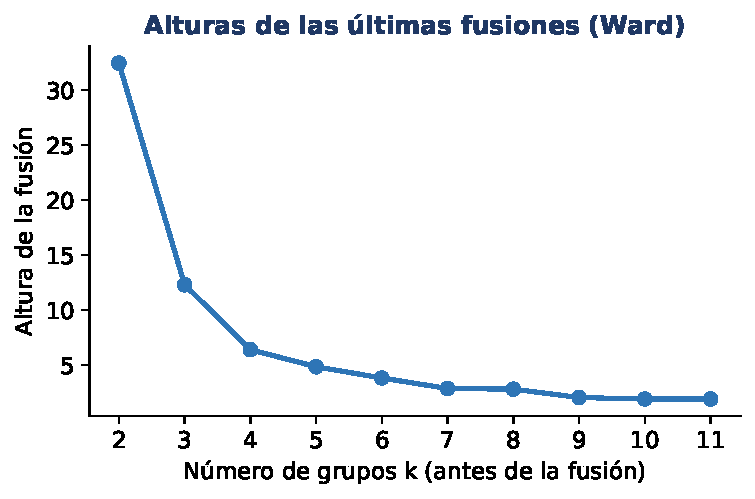
\includegraphics[width=\textwidth]{iris_alturas}
    \column{0.47\textwidth}
    \small
    Alturas de las últimas fusiones:
    2.87, 3.83, 4.85, 6.40, 12.30, 32.45.
    \begin{itemize}
      \item El salto más grande (de 12.3 a 32.5) está en la última fusión: el corte más claro deja \textbf{2 grupos}.
      \item El siguiente salto (de 6.4 a 12.3) sugiere \textbf{3 grupos}.
      \item Las dos escalas de Iris aparecen en un solo árbol: es la ambigüedad entre $k=2$ y $k=3$ de la Sesión 2.
    \end{itemize}
  \end{columns}
\end{frame}

\begin{frame}[fragile]{Paso 3: comparar los criterios de enlace}
\begin{lstlisting}
from sklearn.metrics import adjusted_rand_score
for metodo in ["single", "complete", "average", "ward"]:
    Z_m = linkage(X, method=metodo)
    c, _ = cophenet(Z_m, pdist(X))
    z = fcluster(Z_m, t=3, criterion="maxclust")
    print(metodo, round(c, 3), round(adjusted_rand_score(especie, z), 3), np.bincount(z)[1:])
\end{lstlisting}
  \begin{columns}[c]
    \column{0.42\textwidth}
    \small
    \begin{tabular}{@{}lccc@{}}
      \toprule
      \textbf{Enlace} & \textbf{Cofen.} & \textbf{ARI} & \textbf{Tamaños}\\
      \midrule
      Simple   & 0.86 & 0.56 & 98, 50, 2 \\
      Completo & 0.73 & 0.64 & 72, 50, 28 \\
      Promedio & 0.88 & 0.76 & 64, 50, 36 \\
      Ward     & 0.87 & 0.73 & 64, 50, 36 \\
      \bottomrule
    \end{tabular}\\[4pt]
    {\scriptsize Cofen.: correlación cofenética. ARI: índice de Rand ajustado contra la especie (Sesión 6), con $k=3$.}
    \column{0.56\textwidth}
    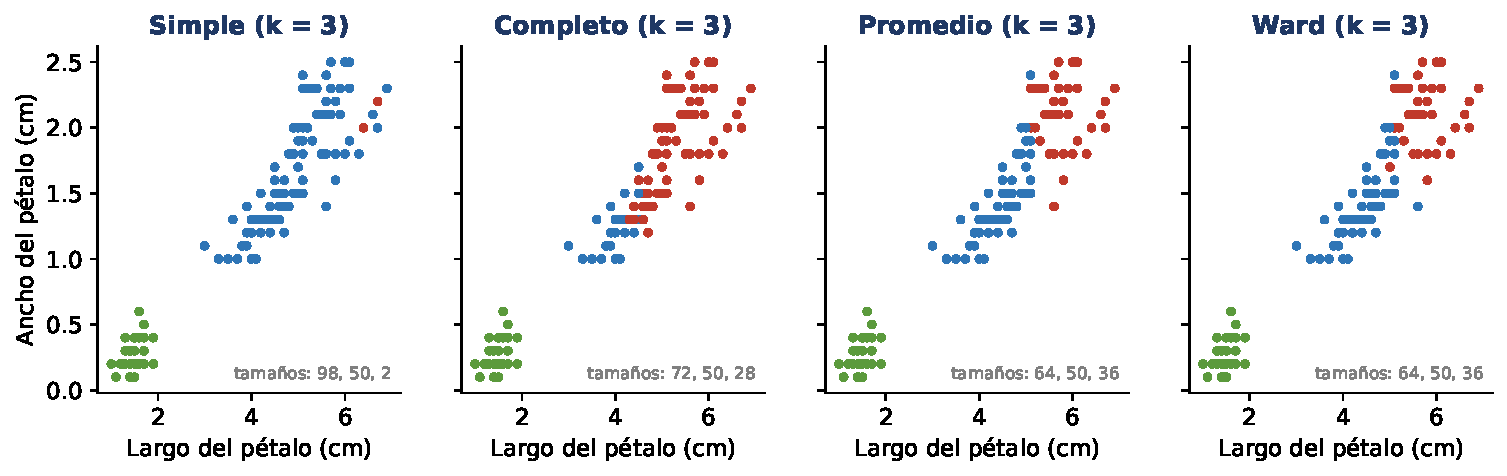
\includegraphics[width=\textwidth]{iris_enlaces}
  \end{columns}
\end{frame}

\begin{frame}{Paso 3: qué muestran los enlaces}
  \begin{itemize}
    \item \textbf{Simple}: separa setosa, pero con $k=3$ el tercer grupo tiene sólo 2 flores.
          Versicolor y virginica quedan encadenadas en un grupo de 98.
    \item \textbf{Completo}: con $k=2$ junta a setosa con 27 versicolor; con $k=3$ la aísla,
          pero parte versicolor en dos (23 y 27). Su correlación cofenética es la más baja (0.73).
    \item \textbf{Promedio} y \textbf{Ward}: tres grupos de 50, 64 y 36 flores, los más
          parecidos a las especies.
    \item El enlace promedio tiene la mayor correlación cofenética (0.88) y la mayor
          coincidencia con las especies (0.76).
  \end{itemize}
  \vspace{6pt}
  \begin{alertblock}{Lección}
    El criterio de enlace cambia el resultado tanto como el algoritmo. La correlación
    cofenética permite compararlos sin usar etiquetas.
  \end{alertblock}
\end{frame}

\begin{frame}{Paso 4: leer el dendrograma}
  \centering
  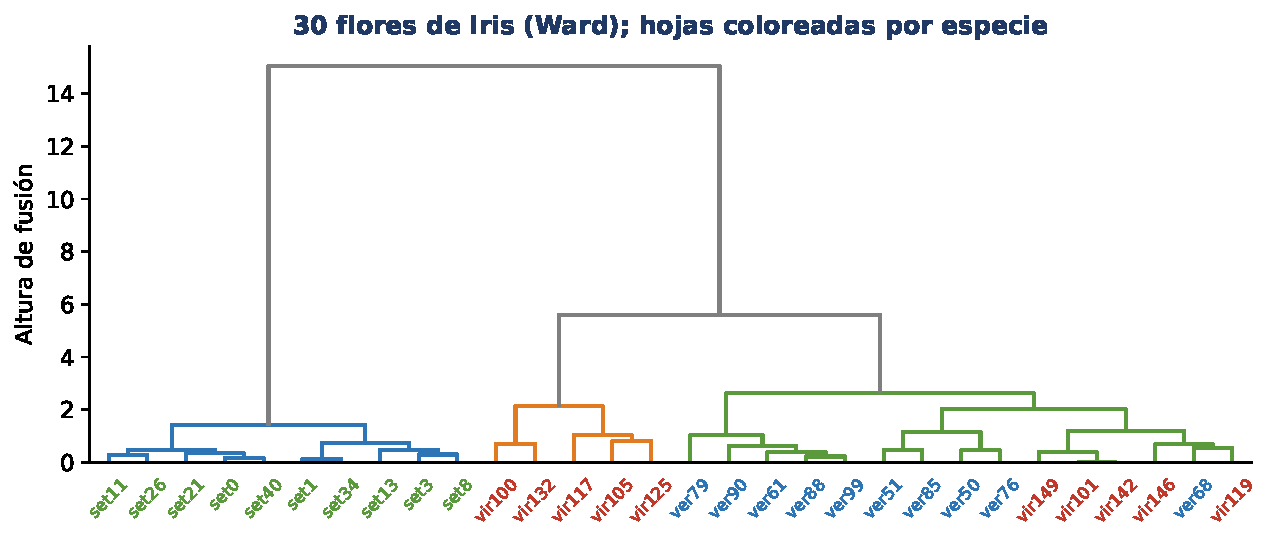
\includegraphics[width=0.72\textwidth]{iris_dendrograma_30}
  \small
  \begin{itemize}
    \item 30 flores, 10 por especie (la especie sólo colorea las hojas). Con 2 grupos: las
          10 setosas, y las 10 versicolor junto con las 10 virginica.
    \item Con 3 grupos: las setosas; 5 virginica; y las 10 versicolor con las otras 5 virginica.
    \item Las virginica que quedan con versicolor son las de pétalos más cortos
          (5.1 cm en promedio, contra 6.2 cm de las otras): se parecen más a versicolor.
  \end{itemize}
\end{frame}

\begin{frame}[fragile]{Paso 5: comparar con k-medias}
\begin{lstlisting}
from sklearn.cluster import KMeans
z_ward = fcluster(linkage(X, "ward"), t=3, criterion="maxclust")
z_km = KMeans(n_clusters=3, n_init=10, random_state=0).fit_predict(X)
print(pd.crosstab(z_ward, z_km))
print(adjusted_rand_score(z_ward, z_km))
\end{lstlisting}
  \begin{columns}[T]
    \column{0.48\textwidth}
    \small
    \begin{block}{Ward contra k-medias ($k=3$)}
      \begin{itemize}
        \item Coinciden en 148 de las 150 flores.
        \item Índice de Rand ajustado entre ambas particiones: 0.96.
        \item Contra la especie: 0.73 los dos.
      \end{itemize}
    \end{block}
    \column{0.48\textwidth}
    \small
    \begin{block}{Ward ($k=3$) contra la especie}
      \centering
      \begin{tabular}{@{}lccc@{}}
        & \textbf{setosa} & \textbf{versic.} & \textbf{virgin.}\\
        \midrule
        Grupo 1 & 50 & 0 & 0 \\
        Grupo 2 & 0 & 1 & 35 \\
        Grupo 3 & 0 & 49 & 15 \\
      \end{tabular}
    \end{block}
  \end{columns}
  \vspace{4pt}
  {\small Ward y k-medias optimizan el mismo criterio (la inercia): Ward lo hace de forma voraz,
  k-medias por iteraciones. Aquí llegan casi a la misma partición.}
\end{frame}

\begin{frame}{Conclusiones del laboratorio}
  \begin{itemize}
    \item Un solo dendrograma muestra las dos escalas de Iris: setosa contra el resto, y después
          versicolor contra virginica.
    \item Los saltos en las alturas de fusión orientan la elección de $k$ sin recalcular nada.
    \item El enlace importa: simple encadena, completo resume mal las distancias, y promedio y Ward
          dan los grupos más útiles.
    \item Ward reproduce casi exactamente el resultado de k-medias, sin depender de una inicialización.
    \item Ningún método separa por completo versicolor y virginica: sus medidas se traslapan.
  \end{itemize}
\end{frame}

%  El mismo código, ejecutado, está en laboratorio_jerarquico.ipynb
% =====================================================================
\section{Laboratorio: agrupamiento jerárquico de Iris}
% =====================================================================

\begin{frame}[fragile]{Paso 1: construir el árbol}
\begin{lstlisting}
import numpy as np, pandas as pd
from sklearn.datasets import load_iris
from scipy.cluster.hierarchy import linkage, dendrogram, fcluster, cophenet
from scipy.spatial.distance import pdist

iris = load_iris()
X, especie = iris.data, iris.target   # medidas en cm; la especie NO se usa para agrupar

Z = linkage(X, method="ward")         # 149 fusiones
dendrogram(Z, no_labels=True)
\end{lstlisting}
  \begin{itemize}
    \item Como en la Sesión 2, se usan las medidas en centímetros sin estandarizar:
          todas tienen la misma unidad y los pétalos son las más informativas.
    \item \texttt{Z} tiene una fila por fusión: los dos grupos unidos, la altura y el tamaño del nuevo grupo.
    \item El dendrograma completo es el de la lámina del problema detonador.
  \end{itemize}
\end{frame}

\begin{frame}[fragile]{Paso 2: dónde cortar}
\begin{lstlisting}
print(Z[-6:, 2].round(2))   # alturas de las 6 ultimas fusiones
\end{lstlisting}
  \begin{columns}[c]
    \column{0.5\textwidth}
    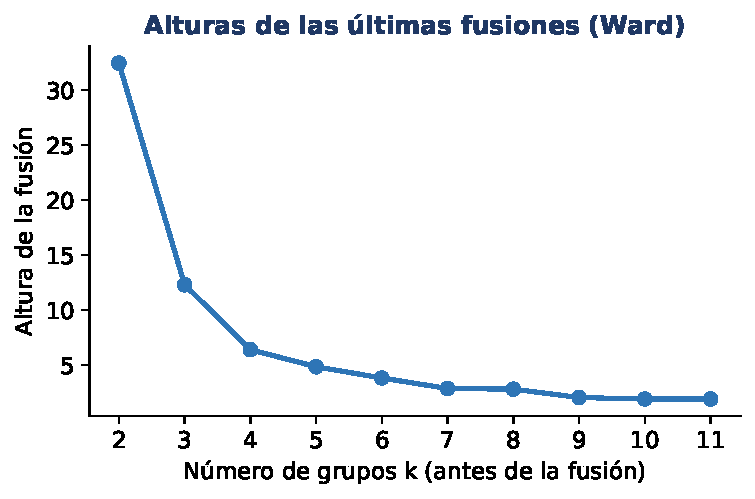
\includegraphics[width=\textwidth]{iris_alturas}
    \column{0.47\textwidth}
    \small
    Alturas de las últimas fusiones:
    2.87, 3.83, 4.85, 6.40, 12.30, 32.45.
    \begin{itemize}
      \item El salto más grande (de 12.3 a 32.5) está en la última fusión: el corte más claro deja \textbf{2 grupos}.
      \item El siguiente salto (de 6.4 a 12.3) sugiere \textbf{3 grupos}.
      \item Las dos escalas de Iris aparecen en un solo árbol: es la ambigüedad entre $k=2$ y $k=3$ de la Sesión 2.
    \end{itemize}
  \end{columns}
\end{frame}

\begin{frame}[fragile]{Paso 3: comparar los criterios de enlace}
\begin{lstlisting}
from sklearn.metrics import adjusted_rand_score
for metodo in ["single", "complete", "average", "ward"]:
    Z_m = linkage(X, method=metodo)
    c, _ = cophenet(Z_m, pdist(X))
    z = fcluster(Z_m, t=3, criterion="maxclust")
    print(metodo, round(c, 3), round(adjusted_rand_score(especie, z), 3), np.bincount(z)[1:])
\end{lstlisting}
  \begin{columns}[c]
    \column{0.42\textwidth}
    \small
    \begin{tabular}{@{}lccc@{}}
      \toprule
      \textbf{Enlace} & \textbf{Cofen.} & \textbf{ARI} & \textbf{Tamaños}\\
      \midrule
      Simple   & 0.86 & 0.56 & 98, 50, 2 \\
      Completo & 0.73 & 0.64 & 72, 50, 28 \\
      Promedio & 0.88 & 0.76 & 64, 50, 36 \\
      Ward     & 0.87 & 0.73 & 64, 50, 36 \\
      \bottomrule
    \end{tabular}\\[4pt]
    {\scriptsize Cofen.: correlación cofenética. ARI: índice de Rand ajustado contra la especie (Sesión 6), con $k=3$.}
    \column{0.56\textwidth}
    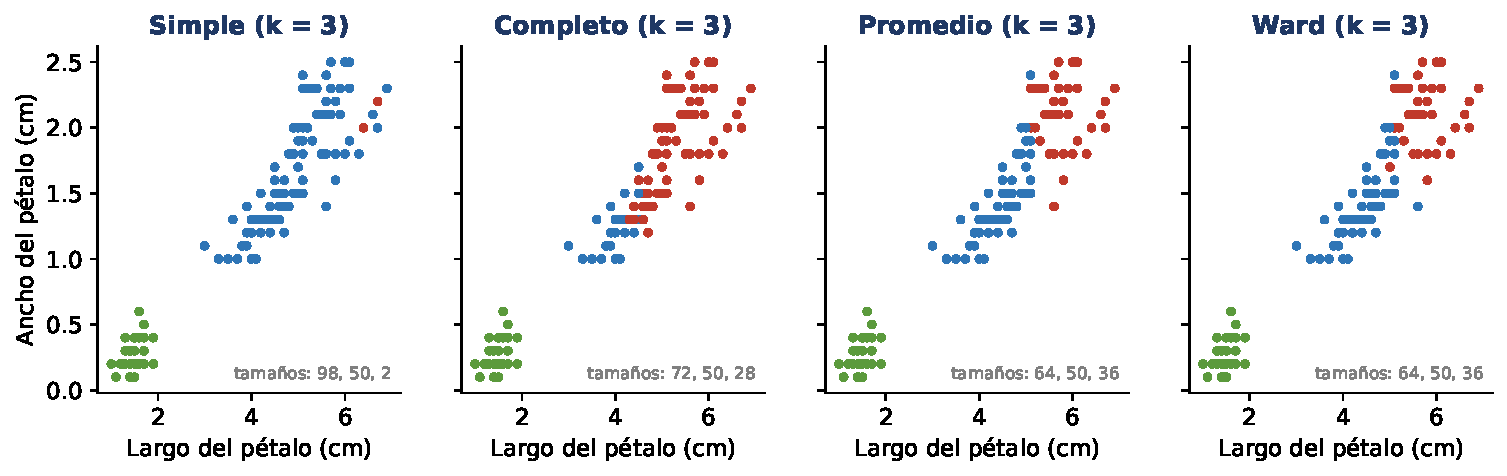
\includegraphics[width=\textwidth]{iris_enlaces}
  \end{columns}
\end{frame}

\begin{frame}{Paso 3: qué muestran los enlaces}
  \begin{itemize}
    \item \textbf{Simple}: separa setosa, pero con $k=3$ el tercer grupo tiene sólo 2 flores.
          Versicolor y virginica quedan encadenadas en un grupo de 98.
    \item \textbf{Completo}: con $k=2$ junta a setosa con 27 versicolor; con $k=3$ la aísla,
          pero parte versicolor en dos (23 y 27). Su correlación cofenética es la más baja (0.73).
    \item \textbf{Promedio} y \textbf{Ward}: tres grupos de 50, 64 y 36 flores, los más
          parecidos a las especies.
    \item El enlace promedio tiene la mayor correlación cofenética (0.88) y la mayor
          coincidencia con las especies (0.76).
  \end{itemize}
  \vspace{6pt}
  \begin{alertblock}{Lección}
    El criterio de enlace cambia el resultado tanto como el algoritmo. La correlación
    cofenética permite compararlos sin usar etiquetas.
  \end{alertblock}
\end{frame}

\begin{frame}{Paso 4: leer el dendrograma}
  \centering
  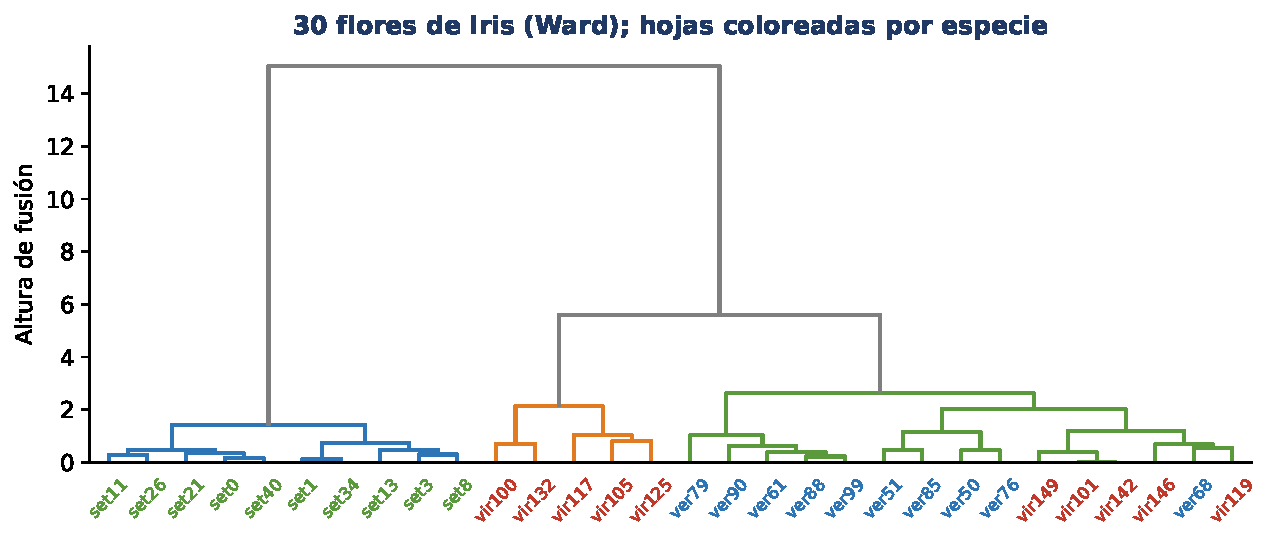
\includegraphics[width=0.72\textwidth]{iris_dendrograma_30}
  \small
  \begin{itemize}
    \item 30 flores, 10 por especie (la especie sólo colorea las hojas). Con 2 grupos: las
          10 setosas, y las 10 versicolor junto con las 10 virginica.
    \item Con 3 grupos: las setosas; 5 virginica; y las 10 versicolor con las otras 5 virginica.
    \item Las virginica que quedan con versicolor son las de pétalos más cortos
          (5.1 cm en promedio, contra 6.2 cm de las otras): se parecen más a versicolor.
  \end{itemize}
\end{frame}

\begin{frame}[fragile]{Paso 5: comparar con k-medias}
\begin{lstlisting}
from sklearn.cluster import KMeans
z_ward = fcluster(linkage(X, "ward"), t=3, criterion="maxclust")
z_km = KMeans(n_clusters=3, n_init=10, random_state=0).fit_predict(X)
print(pd.crosstab(z_ward, z_km))
print(adjusted_rand_score(z_ward, z_km))
\end{lstlisting}
  \begin{columns}[T]
    \column{0.48\textwidth}
    \small
    \begin{block}{Ward contra k-medias ($k=3$)}
      \begin{itemize}
        \item Coinciden en 148 de las 150 flores.
        \item Índice de Rand ajustado entre ambas particiones: 0.96.
        \item Contra la especie: 0.73 los dos.
      \end{itemize}
    \end{block}
    \column{0.48\textwidth}
    \small
    \begin{block}{Ward ($k=3$) contra la especie}
      \centering
      \begin{tabular}{@{}lccc@{}}
        & \textbf{setosa} & \textbf{versic.} & \textbf{virgin.}\\
        \midrule
        Grupo 1 & 50 & 0 & 0 \\
        Grupo 2 & 0 & 1 & 35 \\
        Grupo 3 & 0 & 49 & 15 \\
      \end{tabular}
    \end{block}
  \end{columns}
  \vspace{4pt}
  {\small Ward y k-medias optimizan el mismo criterio (la inercia): Ward lo hace de forma voraz,
  k-medias por iteraciones. Aquí llegan casi a la misma partición.}
\end{frame}

\begin{frame}{Conclusiones del laboratorio}
  \begin{itemize}
    \item Un solo dendrograma muestra las dos escalas de Iris: setosa contra el resto, y después
          versicolor contra virginica.
    \item Los saltos en las alturas de fusión orientan la elección de $k$ sin recalcular nada.
    \item El enlace importa: simple encadena, completo resume mal las distancias, y promedio y Ward
          dan los grupos más útiles.
    \item Ward reproduce casi exactamente el resultado de k-medias, sin depender de una inicialización.
    \item Ningún método separa por completo versicolor y virginica: sus medidas se traslapan.
  \end{itemize}
\end{frame}

%  El mismo código, ejecutado, está en laboratorio_jerarquico.ipynb
% =====================================================================
\section{Laboratorio: agrupamiento jerárquico de Iris}
% =====================================================================

\begin{frame}[fragile]{Paso 1: construir el árbol}
\begin{lstlisting}
import numpy as np, pandas as pd
from sklearn.datasets import load_iris
from scipy.cluster.hierarchy import linkage, dendrogram, fcluster, cophenet
from scipy.spatial.distance import pdist

iris = load_iris()
X, especie = iris.data, iris.target   # medidas en cm; la especie NO se usa para agrupar

Z = linkage(X, method="ward")         # 149 fusiones
dendrogram(Z, no_labels=True)
\end{lstlisting}
  \begin{itemize}
    \item Como en la Sesión 2, se usan las medidas en centímetros sin estandarizar:
          todas tienen la misma unidad y los pétalos son las más informativas.
    \item \texttt{Z} tiene una fila por fusión: los dos grupos unidos, la altura y el tamaño del nuevo grupo.
    \item El dendrograma completo es el de la lámina del problema detonador.
  \end{itemize}
\end{frame}

\begin{frame}[fragile]{Paso 2: dónde cortar}
\begin{lstlisting}
print(Z[-6:, 2].round(2))   # alturas de las 6 ultimas fusiones
\end{lstlisting}
  \begin{columns}[c]
    \column{0.5\textwidth}
    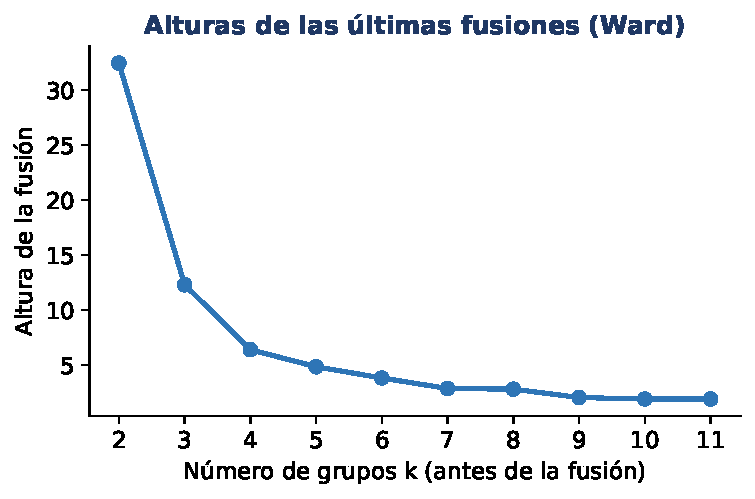
\includegraphics[width=\textwidth]{iris_alturas}
    \column{0.47\textwidth}
    \small
    Alturas de las últimas fusiones:
    2.87, 3.83, 4.85, 6.40, 12.30, 32.45.
    \begin{itemize}
      \item El salto más grande (de 12.3 a 32.5) está en la última fusión: el corte más claro deja \textbf{2 grupos}.
      \item El siguiente salto (de 6.4 a 12.3) sugiere \textbf{3 grupos}.
      \item Las dos escalas de Iris aparecen en un solo árbol: es la ambigüedad entre $k=2$ y $k=3$ de la Sesión 2.
    \end{itemize}
  \end{columns}
\end{frame}

\begin{frame}[fragile]{Paso 3: comparar los criterios de enlace}
\begin{lstlisting}
from sklearn.metrics import adjusted_rand_score
for metodo in ["single", "complete", "average", "ward"]:
    Z_m = linkage(X, method=metodo)
    c, _ = cophenet(Z_m, pdist(X))
    z = fcluster(Z_m, t=3, criterion="maxclust")
    print(metodo, round(c, 3), round(adjusted_rand_score(especie, z), 3), np.bincount(z)[1:])
\end{lstlisting}
  \begin{columns}[c]
    \column{0.42\textwidth}
    \small
    \begin{tabular}{@{}lccc@{}}
      \toprule
      \textbf{Enlace} & \textbf{Cofen.} & \textbf{ARI} & \textbf{Tamaños}\\
      \midrule
      Simple   & 0.86 & 0.56 & 98, 50, 2 \\
      Completo & 0.73 & 0.64 & 72, 50, 28 \\
      Promedio & 0.88 & 0.76 & 64, 50, 36 \\
      Ward     & 0.87 & 0.73 & 64, 50, 36 \\
      \bottomrule
    \end{tabular}\\[4pt]
    {\scriptsize Cofen.: correlación cofenética. ARI: índice de Rand ajustado contra la especie (Sesión 6), con $k=3$.}
    \column{0.56\textwidth}
    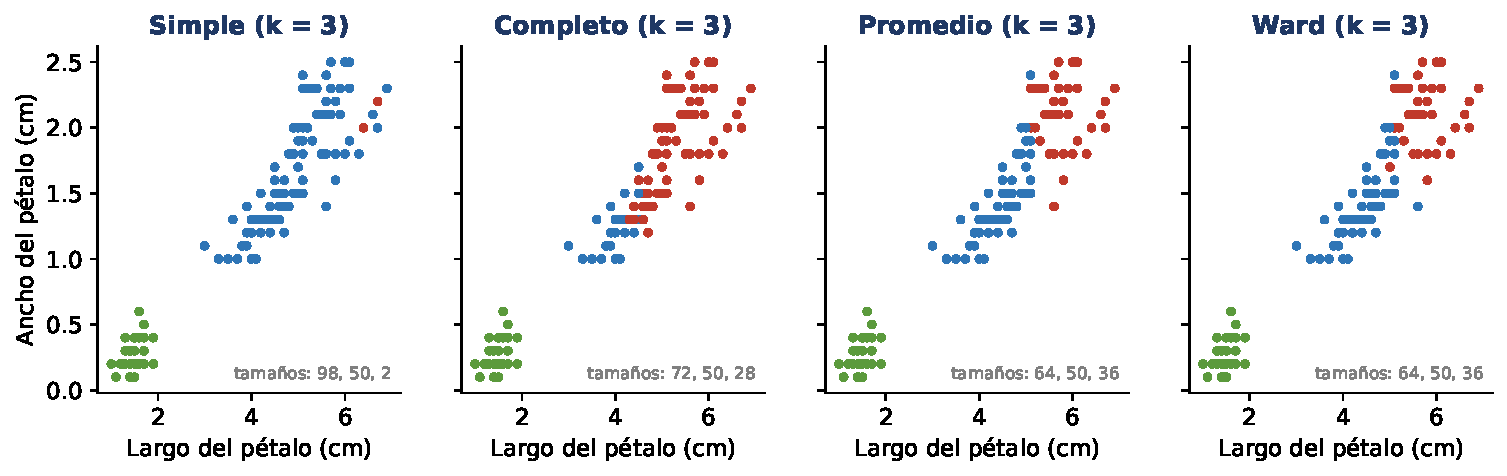
\includegraphics[width=\textwidth]{iris_enlaces}
  \end{columns}
\end{frame}

\begin{frame}{Paso 3: qué muestran los enlaces}
  \begin{itemize}
    \item \textbf{Simple}: separa setosa, pero con $k=3$ el tercer grupo tiene sólo 2 flores.
          Versicolor y virginica quedan encadenadas en un grupo de 98.
    \item \textbf{Completo}: con $k=2$ junta a setosa con 27 versicolor; con $k=3$ la aísla,
          pero parte versicolor en dos (23 y 27). Su correlación cofenética es la más baja (0.73).
    \item \textbf{Promedio} y \textbf{Ward}: tres grupos de 50, 64 y 36 flores, los más
          parecidos a las especies.
    \item El enlace promedio tiene la mayor correlación cofenética (0.88) y la mayor
          coincidencia con las especies (0.76).
  \end{itemize}
  \vspace{6pt}
  \begin{alertblock}{Lección}
    El criterio de enlace cambia el resultado tanto como el algoritmo. La correlación
    cofenética permite compararlos sin usar etiquetas.
  \end{alertblock}
\end{frame}

\begin{frame}{Paso 4: leer el dendrograma}
  \centering
  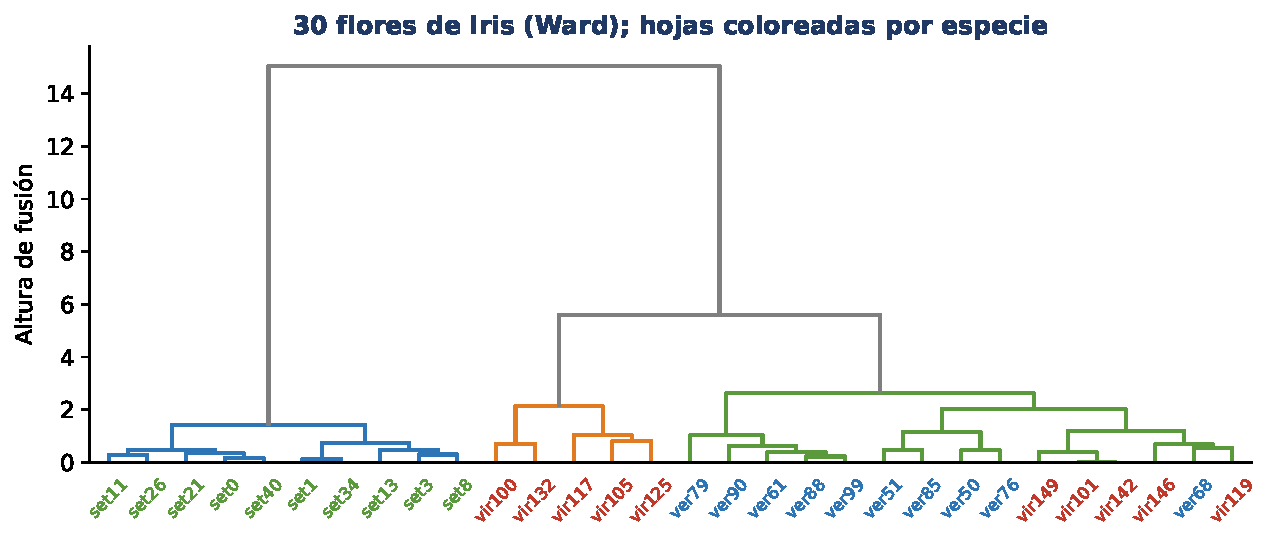
\includegraphics[width=0.72\textwidth]{iris_dendrograma_30}
  \small
  \begin{itemize}
    \item 30 flores, 10 por especie (la especie sólo colorea las hojas). Con 2 grupos: las
          10 setosas, y las 10 versicolor junto con las 10 virginica.
    \item Con 3 grupos: las setosas; 5 virginica; y las 10 versicolor con las otras 5 virginica.
    \item Las virginica que quedan con versicolor son las de pétalos más cortos
          (5.1 cm en promedio, contra 6.2 cm de las otras): se parecen más a versicolor.
  \end{itemize}
\end{frame}

\begin{frame}[fragile]{Paso 5: comparar con k-medias}
\begin{lstlisting}
from sklearn.cluster import KMeans
z_ward = fcluster(linkage(X, "ward"), t=3, criterion="maxclust")
z_km = KMeans(n_clusters=3, n_init=10, random_state=0).fit_predict(X)
print(pd.crosstab(z_ward, z_km))
print(adjusted_rand_score(z_ward, z_km))
\end{lstlisting}
  \begin{columns}[T]
    \column{0.48\textwidth}
    \small
    \begin{block}{Ward contra k-medias ($k=3$)}
      \begin{itemize}
        \item Coinciden en 148 de las 150 flores.
        \item Índice de Rand ajustado entre ambas particiones: 0.96.
        \item Contra la especie: 0.73 los dos.
      \end{itemize}
    \end{block}
    \column{0.48\textwidth}
    \small
    \begin{block}{Ward ($k=3$) contra la especie}
      \centering
      \begin{tabular}{@{}lccc@{}}
        & \textbf{setosa} & \textbf{versic.} & \textbf{virgin.}\\
        \midrule
        Grupo 1 & 50 & 0 & 0 \\
        Grupo 2 & 0 & 1 & 35 \\
        Grupo 3 & 0 & 49 & 15 \\
      \end{tabular}
    \end{block}
  \end{columns}
  \vspace{4pt}
  {\small Ward y k-medias optimizan el mismo criterio (la inercia): Ward lo hace de forma voraz,
  k-medias por iteraciones. Aquí llegan casi a la misma partición.}
\end{frame}

\begin{frame}{Conclusiones del laboratorio}
  \begin{itemize}
    \item Un solo dendrograma muestra las dos escalas de Iris: setosa contra el resto, y después
          versicolor contra virginica.
    \item Los saltos en las alturas de fusión orientan la elección de $k$ sin recalcular nada.
    \item El enlace importa: simple encadena, completo resume mal las distancias, y promedio y Ward
          dan los grupos más útiles.
    \item Ward reproduce casi exactamente el resultado de k-medias, sin depender de una inicialización.
    \item Ningún método separa por completo versicolor y virginica: sus medidas se traslapan.
  \end{itemize}
\end{frame}

%  El mismo código, ejecutado, está en laboratorio_jerarquico.ipynb
% =====================================================================
\section{Laboratorio: agrupamiento jerárquico de Iris}
% =====================================================================

\begin{frame}[fragile]{Paso 1: construir el árbol}
\begin{lstlisting}
import numpy as np, pandas as pd
from sklearn.datasets import load_iris
from scipy.cluster.hierarchy import linkage, dendrogram, fcluster, cophenet
from scipy.spatial.distance import pdist

iris = load_iris()
X, especie = iris.data, iris.target   # medidas en cm; la especie NO se usa para agrupar

Z = linkage(X, method="ward")         # 149 fusiones
dendrogram(Z, no_labels=True)
\end{lstlisting}
  \begin{itemize}
    \item Como en la Sesión 2, se usan las medidas en centímetros sin estandarizar:
          todas tienen la misma unidad y los pétalos son las más informativas.
    \item \texttt{Z} tiene una fila por fusión: los dos grupos unidos, la altura y el tamaño del nuevo grupo.
    \item El dendrograma completo es el de la lámina del problema detonador.
  \end{itemize}
\end{frame}

\begin{frame}[fragile]{Paso 2: dónde cortar}
\begin{lstlisting}
print(Z[-6:, 2].round(2))   # alturas de las 6 ultimas fusiones
\end{lstlisting}
  \begin{columns}[c]
    \column{0.5\textwidth}
    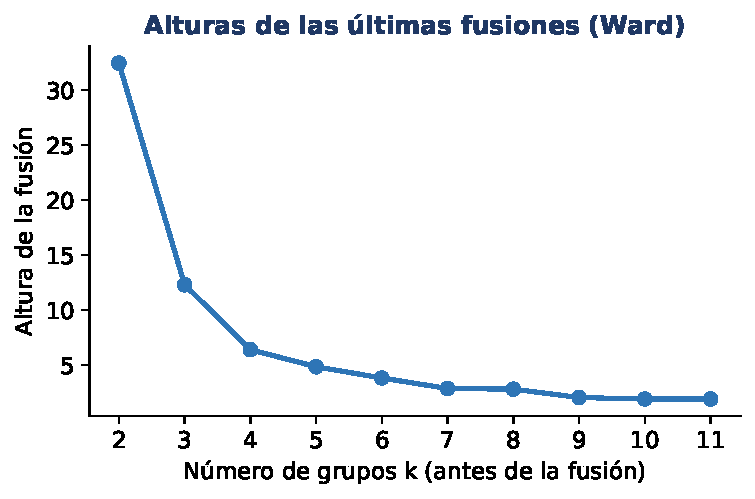
\includegraphics[width=\textwidth]{iris_alturas}
    \column{0.47\textwidth}
    \small
    Alturas de las últimas fusiones:
    2.87, 3.83, 4.85, 6.40, 12.30, 32.45.
    \begin{itemize}
      \item El salto más grande (de 12.3 a 32.5) está en la última fusión: el corte más claro deja \textbf{2 grupos}.
      \item El siguiente salto (de 6.4 a 12.3) sugiere \textbf{3 grupos}.
      \item Las dos escalas de Iris aparecen en un solo árbol: es la ambigüedad entre $k=2$ y $k=3$ de la Sesión 2.
    \end{itemize}
  \end{columns}
\end{frame}

\begin{frame}[fragile]{Paso 3: comparar los criterios de enlace}
\begin{lstlisting}
from sklearn.metrics import adjusted_rand_score
for metodo in ["single", "complete", "average", "ward"]:
    Z_m = linkage(X, method=metodo)
    c, _ = cophenet(Z_m, pdist(X))
    z = fcluster(Z_m, t=3, criterion="maxclust")
    print(metodo, round(c, 3), round(adjusted_rand_score(especie, z), 3), np.bincount(z)[1:])
\end{lstlisting}
  \begin{columns}[c]
    \column{0.42\textwidth}
    \small
    \begin{tabular}{@{}lccc@{}}
      \toprule
      \textbf{Enlace} & \textbf{Cofen.} & \textbf{ARI} & \textbf{Tamaños}\\
      \midrule
      Simple   & 0.86 & 0.56 & 98, 50, 2 \\
      Completo & 0.73 & 0.64 & 72, 50, 28 \\
      Promedio & 0.88 & 0.76 & 64, 50, 36 \\
      Ward     & 0.87 & 0.73 & 64, 50, 36 \\
      \bottomrule
    \end{tabular}\\[4pt]
    {\scriptsize Cofen.: correlación cofenética. ARI: índice de Rand ajustado contra la especie (Sesión 6), con $k=3$.}
    \column{0.56\textwidth}
    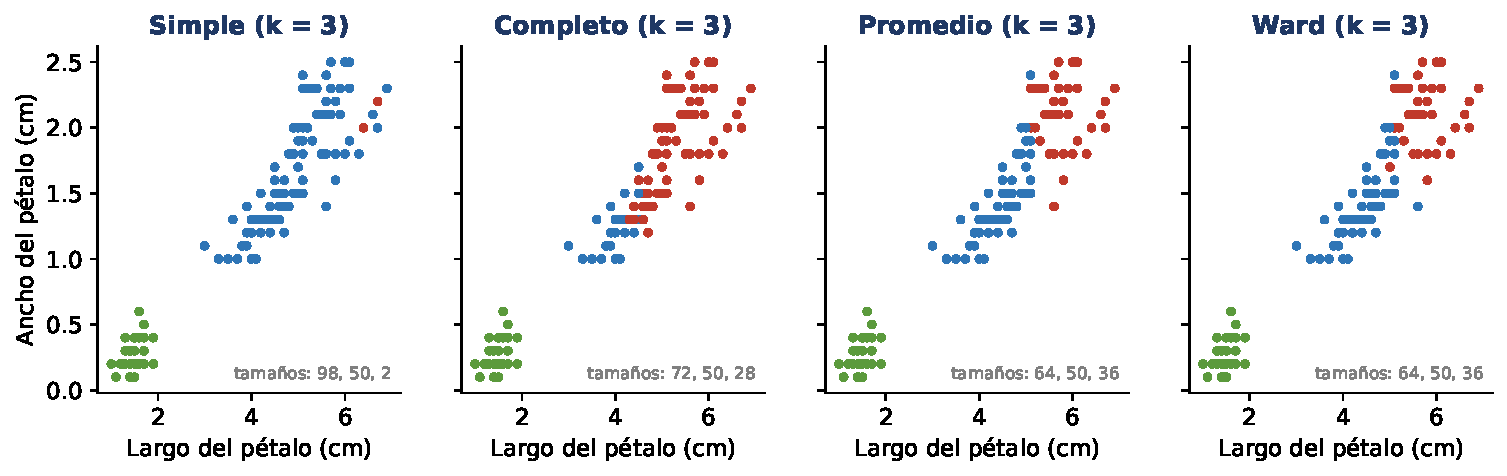
\includegraphics[width=\textwidth]{iris_enlaces}
  \end{columns}
\end{frame}

\begin{frame}{Paso 3: qué muestran los enlaces}
  \begin{itemize}
    \item \textbf{Simple}: separa setosa, pero con $k=3$ el tercer grupo tiene sólo 2 flores.
          Versicolor y virginica quedan encadenadas en un grupo de 98.
    \item \textbf{Completo}: con $k=2$ junta a setosa con 27 versicolor; con $k=3$ la aísla,
          pero parte versicolor en dos (23 y 27). Su correlación cofenética es la más baja (0.73).
    \item \textbf{Promedio} y \textbf{Ward}: tres grupos de 50, 64 y 36 flores, los más
          parecidos a las especies.
    \item El enlace promedio tiene la mayor correlación cofenética (0.88) y la mayor
          coincidencia con las especies (0.76).
  \end{itemize}
  \vspace{6pt}
  \begin{alertblock}{Lección}
    El criterio de enlace cambia el resultado tanto como el algoritmo. La correlación
    cofenética permite compararlos sin usar etiquetas.
  \end{alertblock}
\end{frame}

\begin{frame}{Paso 4: leer el dendrograma}
  \centering
  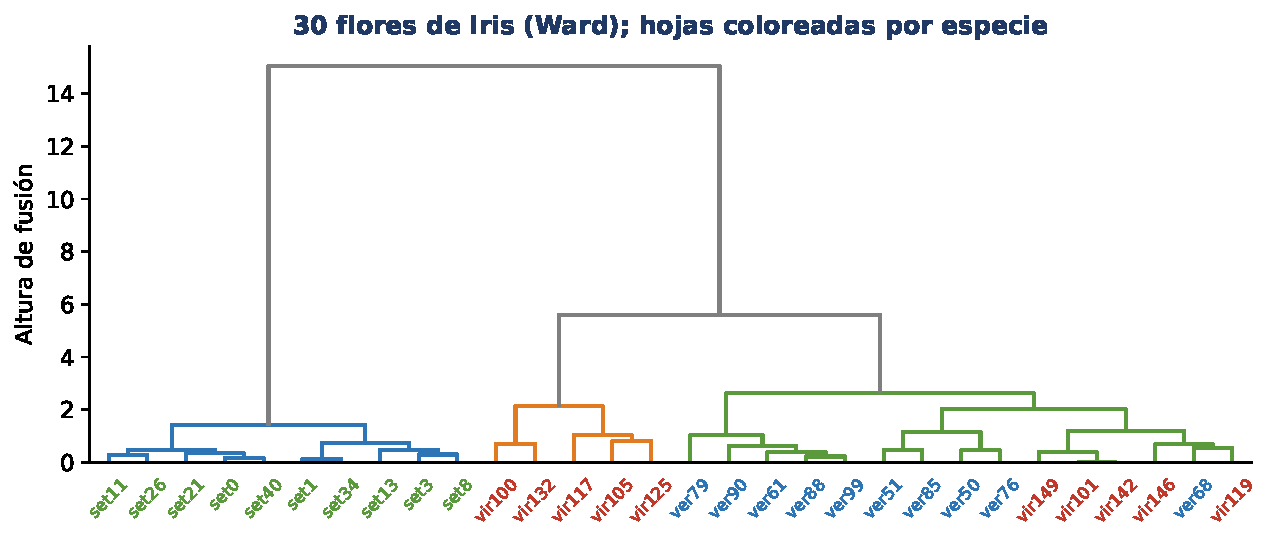
\includegraphics[width=0.72\textwidth]{iris_dendrograma_30}
  \small
  \begin{itemize}
    \item 30 flores, 10 por especie (la especie sólo colorea las hojas). Con 2 grupos: las
          10 setosas, y las 10 versicolor junto con las 10 virginica.
    \item Con 3 grupos: las setosas; 5 virginica; y las 10 versicolor con las otras 5 virginica.
    \item Las virginica que quedan con versicolor son las de pétalos más cortos
          (5.1 cm en promedio, contra 6.2 cm de las otras): se parecen más a versicolor.
  \end{itemize}
\end{frame}

\begin{frame}[fragile]{Paso 5: comparar con k-medias}
\begin{lstlisting}
from sklearn.cluster import KMeans
z_ward = fcluster(linkage(X, "ward"), t=3, criterion="maxclust")
z_km = KMeans(n_clusters=3, n_init=10, random_state=0).fit_predict(X)
print(pd.crosstab(z_ward, z_km))
print(adjusted_rand_score(z_ward, z_km))
\end{lstlisting}
  \begin{columns}[T]
    \column{0.48\textwidth}
    \small
    \begin{block}{Ward contra k-medias ($k=3$)}
      \begin{itemize}
        \item Coinciden en 148 de las 150 flores.
        \item Índice de Rand ajustado entre ambas particiones: 0.96.
        \item Contra la especie: 0.73 los dos.
      \end{itemize}
    \end{block}
    \column{0.48\textwidth}
    \small
    \begin{block}{Ward ($k=3$) contra la especie}
      \centering
      \begin{tabular}{@{}lccc@{}}
        & \textbf{setosa} & \textbf{versic.} & \textbf{virgin.}\\
        \midrule
        Grupo 1 & 50 & 0 & 0 \\
        Grupo 2 & 0 & 1 & 35 \\
        Grupo 3 & 0 & 49 & 15 \\
      \end{tabular}
    \end{block}
  \end{columns}
  \vspace{4pt}
  {\small Ward y k-medias optimizan el mismo criterio (la inercia): Ward lo hace de forma voraz,
  k-medias por iteraciones. Aquí llegan casi a la misma partición.}
\end{frame}

\begin{frame}{Conclusiones del laboratorio}
  \begin{itemize}
    \item Un solo dendrograma muestra las dos escalas de Iris: setosa contra el resto, y después
          versicolor contra virginica.
    \item Los saltos en las alturas de fusión orientan la elección de $k$ sin recalcular nada.
    \item El enlace importa: simple encadena, completo resume mal las distancias, y promedio y Ward
          dan los grupos más útiles.
    \item Ward reproduce casi exactamente el resultado de k-medias, sin depender de una inicialización.
    \item Ningún método separa por completo versicolor y virginica: sus medidas se traslapan.
  \end{itemize}
\end{frame}
